\documentclass{article}
\usepackage{graphicx} % Required for inserting images
\usepackage{float}
\usepackage{amsmath}

\title{ECE148: Signal Processing Applications \\ \large 
Assignment 5: Hilbert Transform}
\author{Andy Chen}
\date{May 2026}

\begin{document}

\maketitle

\section{Introduction}
Consider a real and periodic signal \(f(t)\), of period \(T\). The signal has 7 harmonics for \(m = 1, 2, ..., 7\).
\[
f(t) = \sum_{m=1}^{7} a_m \cos\bigg( \frac{2\pi mt}{T}\bigg)
\]
The 7 coefficients \(a_m\) are formed with my personal 7-digit UCSB perm number, \([1, 0, 5, 5, 3, 8, 8]\).

\section{Method A: Hilbert Transform and Sampling}
\subsection*{Hilbert Transform of \(f(t)\)}
The Hilbert transform of \(\cos(\omega t)\) is:
\[
\mathcal{H} \{\cos(\omega t) \} = \sin(\omega t)
\]
Therefore, the Hilbert transform of the periodic function \(f(t)\) is:
\[
\hat{f}(t) = \sum_{m=1}^{7} a_m \sin\bigg( \frac{2\pi mt}{T}\bigg)
\]
\begin{figure}[H]
    \centering
    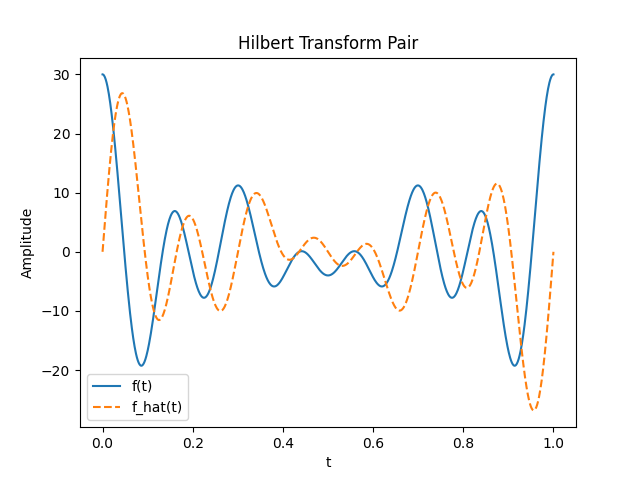
\includegraphics[width=1\linewidth]{hilberttransformpair.png}
    \caption{Hilbert transform pair, \(f(t)\) and \(\hat{f}(t)\), from \(t=0\) to \(t=T\).}
    \label{fig:placeholder}
\end{figure}

\subsection*{Fourier Series Expansion}
Using the identities:
\[
\cos(\omega t) = \frac{1}{2} (e^{j\omega t} + e^{-j\omega t})
\]
\[
\sin(\omega t) = \frac{1}{2j} (e^{j\omega t} - e^{-j\omega t})
\]
We can formulate both \(f(t)\) and \(\hat{f}(t)\) in the form of complex Fourier series expansion:
\[
f(t) = \sum_{m=1}^{7} \frac{a_m}{2} e^{j2\pi mt/T} + \sum_{m=1}^{7} \frac{a_m}{2} e^{-j2\pi mt/T}
\]
\[
\hat{f}(t) = \sum_{m=1}^{7} \frac{a_m}{2j} e^{j2\pi mt/T} - \sum_{m=1}^{7} \frac{a_m}{2j} e^{-j2\pi mt/T}
\]
\(f(t)\) will have complex coefficients \(C_m = C_{-m} = \frac{a_m}{2j}\). \(\hat{f}(t)\) will have complex coefficients \(C_m = \frac{a_m}{2j}\) and \(C_{-m} = -\frac{a_m}{2j}\).

\subsection*{Orthogonality and Equal Power}
\(f(t)\) is an even function whereas \(\hat{f}(t)\) is an odd function. An odd function multiplied by an even function is an odd function. The integral of an odd function over one period is zero. Therefore, \(f(t)\) and \(\hat{f}(t)\) are orthogonal.
\[
\int_{0}^{T} f(t) \hat{f}(t) dt = 0
\]
Using Parseval's theorem, we have:
\[
\int_{-\infty}^{\infty} |f(t)|^2 dt = \int_{-\infty}^{\infty} f(t) \ f^*(t) dt
= \frac{1}{2\pi}\int_{-\infty}^{\infty} F(j\omega) \ F^*(j\omega) d\omega
\]
In the frequency domain, \(\hat{F}(j\omega) = -j sgn \ F(j\omega)\). Using Parseval's, we have:
\[
\int_{-\infty}^{\infty} |\hat{f}(t)|^2 dt = \int_{-\infty}^{\infty} \hat{f}(t) \ \hat{f}^*(t) dt
= \frac{1}{2\pi}\int_{-\infty}^{\infty} \hat{F}(j\omega) \ \hat{F}^*(j\omega) d\omega
\]
\[
= \frac{1}{2\pi}\int_{-\infty}^{\infty} (-j sgn(\omega))F(j\omega) \ (jsgn(\omega))F^*(j\omega)d\omega
\]
\[
= \frac{1}{2\pi}\int_{-\infty}^{\infty} F(j\omega) \ F^*(j\omega) d\omega
\]
Thus, the energies of both signals are the same. In this case, both energies sum to 1504.

\subsection*{16-Point Sampling}
Given \(\Delta t = \frac{T}{16}\) for \(n=0, 1, 2, ...15\), we have:
\[
f[n] = f(n\Delta t) = \sum_{m=1}^{7}a_m \cos\bigg(\frac{2\pi m}{16}n\bigg)
\]
\[
\hat{f}[n] = \hat{f}(n\Delta t) = \sum_{m=1}^{7}a_m \sin\bigg(\frac{2\pi m}{16}n\bigg)
\]
We check for orthogonality:
\[
\sum_{n=0}^{15} f[n] \ \hat{f}[n] = \sum_{m=1}^{7} \sum_{k=1}^{7} a_m a_k \sum_{n=0}^{15} 
\cos\bigg(\frac{2\pi m}{16}n \bigg) \sin\bigg(\frac{2\pi k}{16}n \bigg)
\]
For integer harmonics over one full period, 
\[
\sum_{n=0}^{15} \cos\bigg(\frac{2\pi m}{16}n \bigg) \sin\bigg(\frac{2\pi k}{16}n \bigg) = 0
\]
Thus, we have \(f[n]\) and \(\hat{f}[n]\) are orthogonal. We solve for the discrete energy of \(f[n]\):
\[
\sum_{n=0}^{15} |f[n]|^2 = \sum_{m,k} a_m a_k\sum_{n=0}^{15} 
\cos\bigg(\frac{2\pi m}{16}n \bigg) \cos\bigg(\frac{2\pi k}{16}n \bigg)
\]
Using cosine orthogonality, we find that the sum of the two cosines is 8 when \(m=k\). Therefore, we have the energy:
\[
E_f = 8\sum_{m=1}^{7}a^2_m = 1504
\]
Similarly, using sine orthogonality and solving for the discrete energy of \(\hat{f}(t)\) yields:
\[
E_{\hat{f}} = 8\sum_{m=1}^{7} a^2_m = 1504
\]

\subsection*{Analytic Signal and DFT}
We form the analytic sequence \(\tilde{f}[n] = f[n] + j\hat{f}[n] \):
\[
\tilde{f}[n] = \sum_{m=1}^{7}a_m \cos\bigg(\frac{2\pi m}{16}n\bigg)
+ j\sum_{m=1}^{7}a_m \sin\bigg(\frac{2\pi m}{16}n\bigg)
\]
Using complex exponentials, we have:
\[
\tilde{f}[n] = \sum_{m=1}^{7} a_m e^{j\frac{2\pi n}{16}m}
\]
We solve for the DFT:
\[
\tilde{F}[k] = \sum_{m=1}^{7} a_m \sum_{n=0}^{15}e^{j\frac{2\pi n}{16}m} e^{-j\frac{2\pi n}{16}k}
\]
\[
\tilde{F}[k] = \sum_{m=1}^{7} a_m \sum_{n=0}^{15}e^{-j\frac{2\pi n}{16}(k-m)}
\]
Thus, we have the resultant DFT spectral sequence:
\[
[0,\ 16,\ 0,\ 80,\ 80,\ 48,\ 128,\ 128,\ 0,\ 0,\ 0,\ 0,\ 0,\ 0,\ 0,\ 0]
\]

\subsection*{Comparison of \(\tilde{F}(k)\) to the 7-point sequence \(a_m\)}
In the continuous-time domain, the original 7-point sequence \(\{a_m\}\) represents the amplitude of the cosine harmonics. The 16-point result \(\tilde{F}[k]\) is directly related to \(a_m\) by the relationship:
\[
\tilde{F}[k] = \begin{cases}
    16a_k & k =1,...,7 \\
    0 & \text{otherwise}
\end{cases}
\]
From the Fourier series expansion, we see that energy is split between \(+m\) and \(-m\), where each side has \(\frac{a_m}{2}\). After applying the Hilbert transform and combining the transform pair to form the 16-point complex analytic sequence, we find that the negative frequencies are removed and positive frequencies become full amplitude \(a_m\). Taking the DFT recovers those amplitudes exactly (scaled by 16).

\section{Method B: Sampling and Hilbert Transform}
\subsection*{Sampling \(f(t)\)}
We take 16 uniform samples of \(f(t)\) within one period with sample spacing \(\Delta t = \frac{T}{16}\) to form a 16-point sequence \(f[n] = f(n\Delta t)\), where \(n=0,1,2,...,15\).
\[
f[n] = f(n\Delta t) = \sum_{m=1}^{7}a_m \cos\bigg(\frac{2\pi m}{16}n\bigg)
\]
\begin{figure}[H]
    \centering
    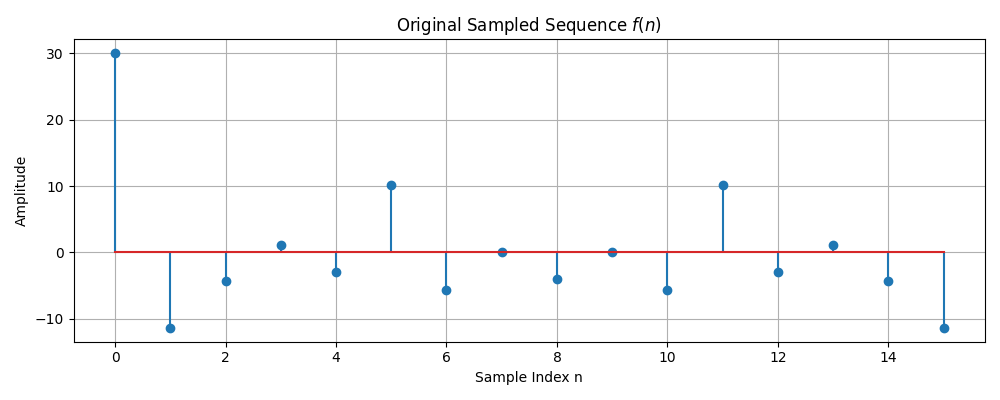
\includegraphics[width=1\linewidth]{originalsampledsequence.png}
    \caption{The 16-point sequence \(f[n]\).}
    \label{fig:placeholder}
\end{figure}

\subsection*{Hilbert Transform with 16-Point FFT}
The FFT of \(f[n]\) is:
\[
F[k] = \sum_{m=1}^{7}a_m \sum_{n=0}^{15} \cos\bigg(\frac{2\pi m}{16}n\bigg)  e^{-j\frac{2\pi n}{16} k}
\]
From the FFT, we can use the following identity to derive the FFT of the Hilbert transform.
\[
\hat{F}[k] = -j sgn(k) \ F[k]
\]
\[
\hat{F}[k] = -jsgn(k) \ \sum_{m=1}^{7}a_m \sum_{n=0}^{15} \cos\bigg(\frac{2\pi m}{16}n\bigg)  e^{-j\frac{2\pi n}{16} k}
\]
Taking the inverse DFT yields the discrete-time Hilbert transform \(\hat{f}[n]\):
\[
\hat{f}[n] = \sum_{m=1}^{7}a_m \sin\bigg(\frac{2\pi m}{16}n\bigg)
\]
\begin{figure} [H]
    \centering
    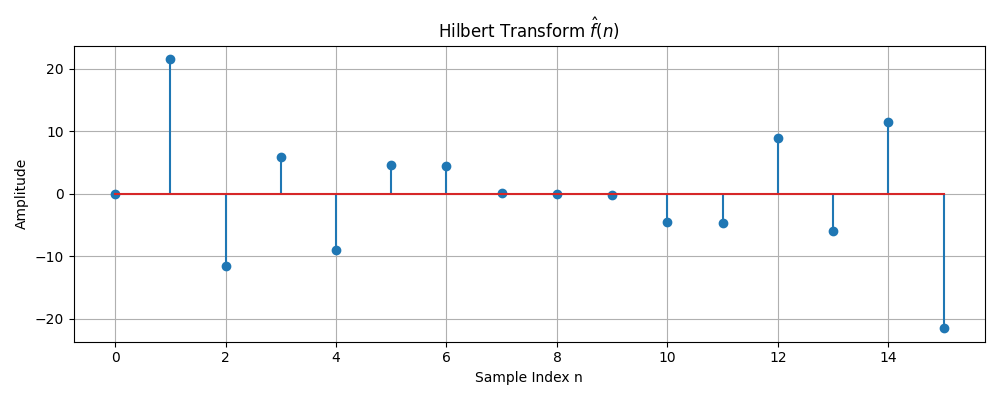
\includegraphics[width=1\linewidth]{hilberttransformfn.png}
    \caption{Hilbert Transform of \(f[n].\)}
    \label{fig:placeholder}
\end{figure}

\subsection*{Orthogonality and Equal Power}
We check the Hilbert transform pair's orthogonality by calculating the inner product:
\[
\sum_{n=0}^{15} f[n] \hat{f}[n]
\]
The inner product of the pair is 0 as the cosine and sine components are orthogonal to each other. Therefore, \(f[n]\) and \(\hat{f}[n]\) are orthogonal. 
The discrete energy of the original sequence and the Hilbert transform are given as:
\[
E_f = \sum_{n=0}^{15} |f[n]|^2
\]
\[
E_{\hat{f}} = \sum_{n=0}^{15} |\hat{f}[n]|^2
\]
Repeating the same calculations from before, we find that:
\[
E_f = E_{\hat{f}} = \sum_{m=1}^{7}a_m^2 = 1504
\]
Thus, the total energy levels of \(f[n]\) and \(\hat{f}[n]\) are equal to each other.

\subsection*{Analytic Signal and DFT}
Combining the Hilbert transform pair, we form the 16-point complex analytic sequence:
\[
\tilde{f}[n] = \sum_{m=1}^{7}a_m \cos\bigg(\frac{2\pi m}{16}n\bigg)
+ j\sum_{m=1}^{7}a_m \sin\bigg(\frac{2\pi m}{16}n\bigg)
\]
Taking the 16-point DFT/FFT of the analytic sequence \(\tilde{f}[n]\) results in the following spectral sequence:
\[
\tilde{F}[k] = [0, 16, 0, 80, 80, 48, 128, 128, 0, 0, 0, 0, 0, 0, 0, 0]
\]
\begin{figure}[H]
    \centering
    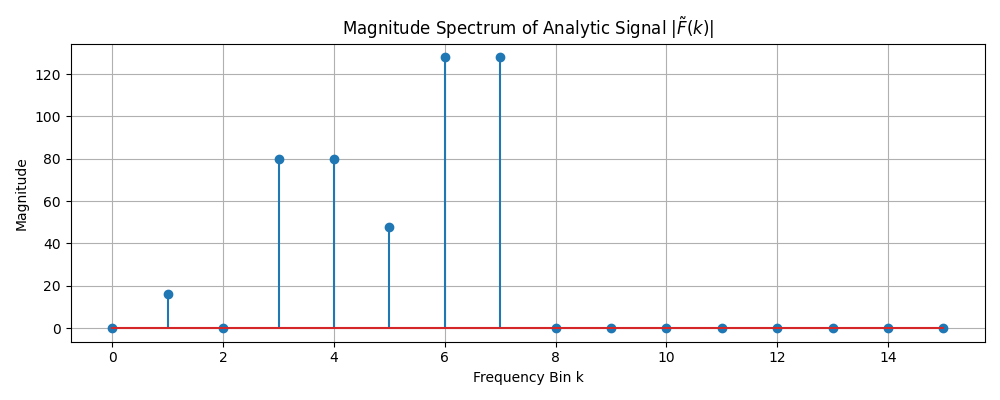
\includegraphics[width=1\linewidth]{magnitudeanalytic.png}
    \caption{Magnitude spectrum of the analytic signal \(\tilde{F}[k].\)}
    \label{fig:placeholder}
\end{figure}
\subsection*{Comparison of \(\tilde{F}[k]\) with Part A}
In Method A, we applied a Hilbert transform in continuous time and then sampled. In Method B, we sampled first and then applied the Hilbert transform via DFT/FFT. Remarkably, both methods resulted in the same \(\tilde{F}[k]\) where:
\[
\tilde{F}[k] = \begin{cases}
    16a_k & k =1,...,7 \\
    0 & \text{otherwise}
\end{cases}
\]
This occurs because the signal is band-limited and sampled exactly over one period, so no aliasing occurs. The FFT-based Hilbert transform correctly removes negative frequency components and preserves positive frequency components, resulting in the same one-sided spectrum where \(\tilde{F}[k] = 16a_k\) for \(k=1,...,7\). 

\end{document}
